\chapter{Cyber-Physical Systems}

\section{Introducción}


\begin{definition}
   [CPS]
   A cyber-physical system is a system of collaborating computational
   elements controlling physical entities
\end{definition}
Cyber-Physical System (CPS) is a generic term for a variety of
control systems, such as SCADA (Supervisory Control and Data
Acquisition) systems, ICSs (Industrial Control Systems), BCSs
(Building Control Systems), and the global electrical smart grid

\begin{definition}
   [CPS - 2]
   A Cyber Physical System (CPS) is a network of interacting and
   collaborating computational elements controlling physical entities,
   including sensors, actuators, control processing units, and
   communication devices
\end{definition}

\begin{definition}
   [CPS - 3]
   CPS are systems used to monitor and control the physical world
\end{definition}

\begin{definition}
   [CPS - 4]
   CPS are IT systems that are integrated into physical world application
\end{definition}

\framedt{Events out of temperatures}{
   Consideremos un escenario en el que se mide la temperatura con un sensor.
   Para saber si la temperatura es alta o baja, se necesita un umbral, lo que se llama un \textbf{valor de referencia}.\\
   Esto permite de comparar la temperatura medida con el valor de referencia y tomar una decisión, como por ejemplo generar una alarma si la temperatura es demasiado alta.
}

\section{Componenetes de CPSs}

CPS tienen vulnerabilidades específicas, porque hay:
\begin{itemize}
	\item Issolation asumption
	\item Increased connectivity
	\item Heterogeneity
	\item Long life cycle of components
	\note{Hay softwares que todavía necesitan Windows XP}
\end{itemize}

\begin{figure}[htbp]
   \centering
   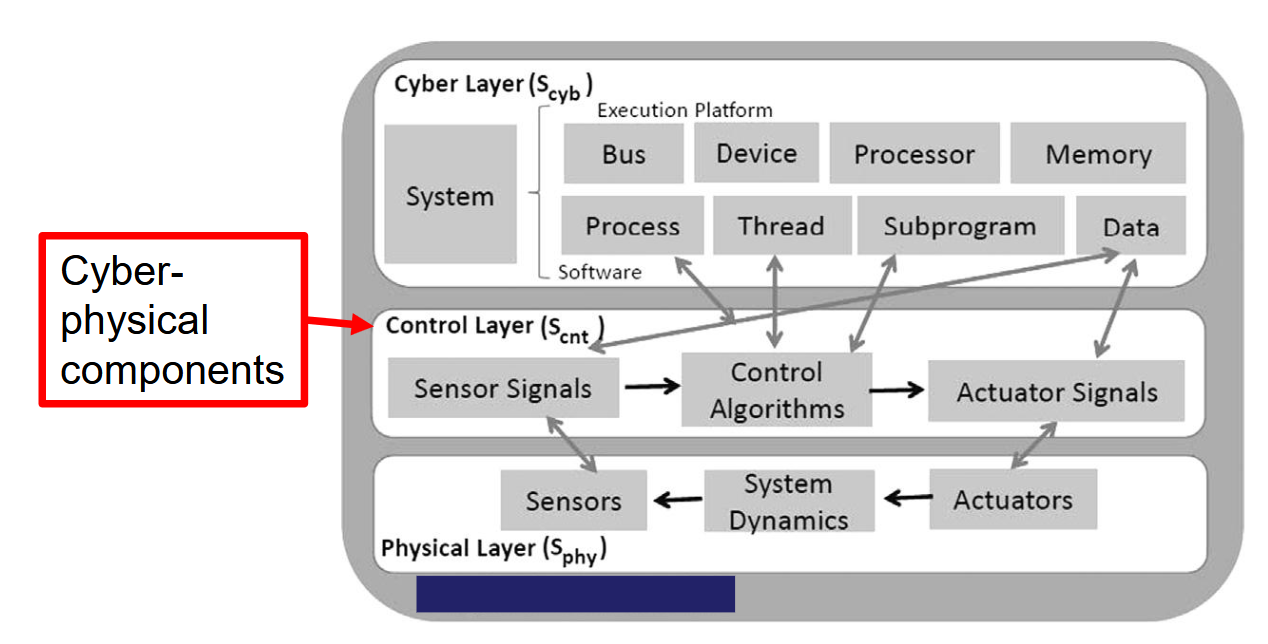
\includegraphics{images/06/CPScomponents.png}
   \caption{Cyberphysical Components}
   \label{fig:06/CPScomponents}
\end{figure}


\subsubsection{Industrial Control Systems}
Sometimes are called SCADA (Supervisory Control and Data Acquisition) systems or DCS (Distributed Control Systems).

El ejemplo más común de ICS son las redes de PLC, por wired o wireless. Tradicionalmente, los PLCs se comunican con un SCADA a través ambos de un protocolo OT (Operational Technologies) de comunicación propietario y de los protocolos IT standard.\\
Tradicionalmente, la isolación era la mejor defensa para estos sistemas.
Patching y updates son un problema, porque los sistemas no pueden ser apagados, y entonces no pueden ser parcheados.

SCADA systems se componen de 4 niveles:
\begin{enumerate}
	\item Sensors and actuators
	\item Distributed controllers, which include programmable logic
   controllers (PLCs), intelligent electronic devices (IEDs), and
   other forms of programmable automation controllers (PACs)
	\item Supervisory and control systems, which encompasses
   systems that store process data, and implements control
   schemes to manage the lower levels
	\item Human machine interfaces (HMIs), which enable the human
   operators to manage the physical process
\end{enumerate}

Diferencias entre ICS y sistemas IT:
\begin{itemize}
	\item Logic execution has a big impact on the physical environtment
	\item Edge devices are, at least, so relevant as hosts servers
	\item Computation resources of edge devices are usually very limited
	\item Safety is the most relevant design constrain
	\item Continuous availability and time-critically constrains
	\item Hard-Real time vs Soft-Real time vs Best-Effort systems
\end{itemize}

SCADA network components:
\begin{itemize}
	\item Servers and workstations that are used by operators to
interact with the field devices segment
	\item HMI software-based graphical user interface
	\item Monitoring of field devices
	\item Field devices data updating
	\item Historian systems
	\item Back up systems (similar to IT systems)
\end{itemize}

Field devices components:
\begin{itemize}
	\item Programmable Logic Controllers (PLCs)
	\item Remote Terminal Units (RTUs)
	\item Intelligent Electronic Devices (IEDs)
	\item IEDs are microprocessor based devices as sensors, motors (actuators),
brakes,lights, etc
	\item IEDs are controled by RTUs and PLCs by mean of field buses
protocols (as PROFIBUS DP)
	\item RTUs monitor IEDs and transmit data to PLCs using ModBUS RTU and
DNP3
	\item Sometimes, directed to the SCADA network using ModBUS TCP
	\item PLCs are control computers, with many types of I/O interfaces
\end{itemize}

Usual incidents in ICSs:
\begin{itemize}
	\item Blocked or delayed flow of information through ICS networks, which could
disrupt ICS operation
	\item Unauthorized changes to instructions, commands, or alarm thresholds, which
could damage, disable, or shut down equipment, create environmental
impacts, and/or endanger human life
	\item Inaccurate information sent to system operators, either to disguise
unauthorized changes, or to cause the operators to initiate inappropriate
actions, which could have various negative effects
	\item ICS software or configuration settings modified, or ICS software infected with
malware, which could have various negative effects
	\item Interference with the operation of equipment protection systems, which could
endanger costly and difficult-to-replace equipment
	\item Interference with the operation of safety systems, which could endanger
human life
\end{itemize}

\section{Vulnerabilidades}
\begin{enumerate}
	\item Vulnerabilities inherent in the CPS product, or platform
vulnerabilities
	\item Vulnerabilities because of poor network design or
configuration, or network equipment vulnerabilities
	\item Vulnerabilities caused during the installation, configuration,
and maintenance of the CPS, or management vulnerabilities
\end{enumerate}

\begin{figure}[htbp]
	\centering
	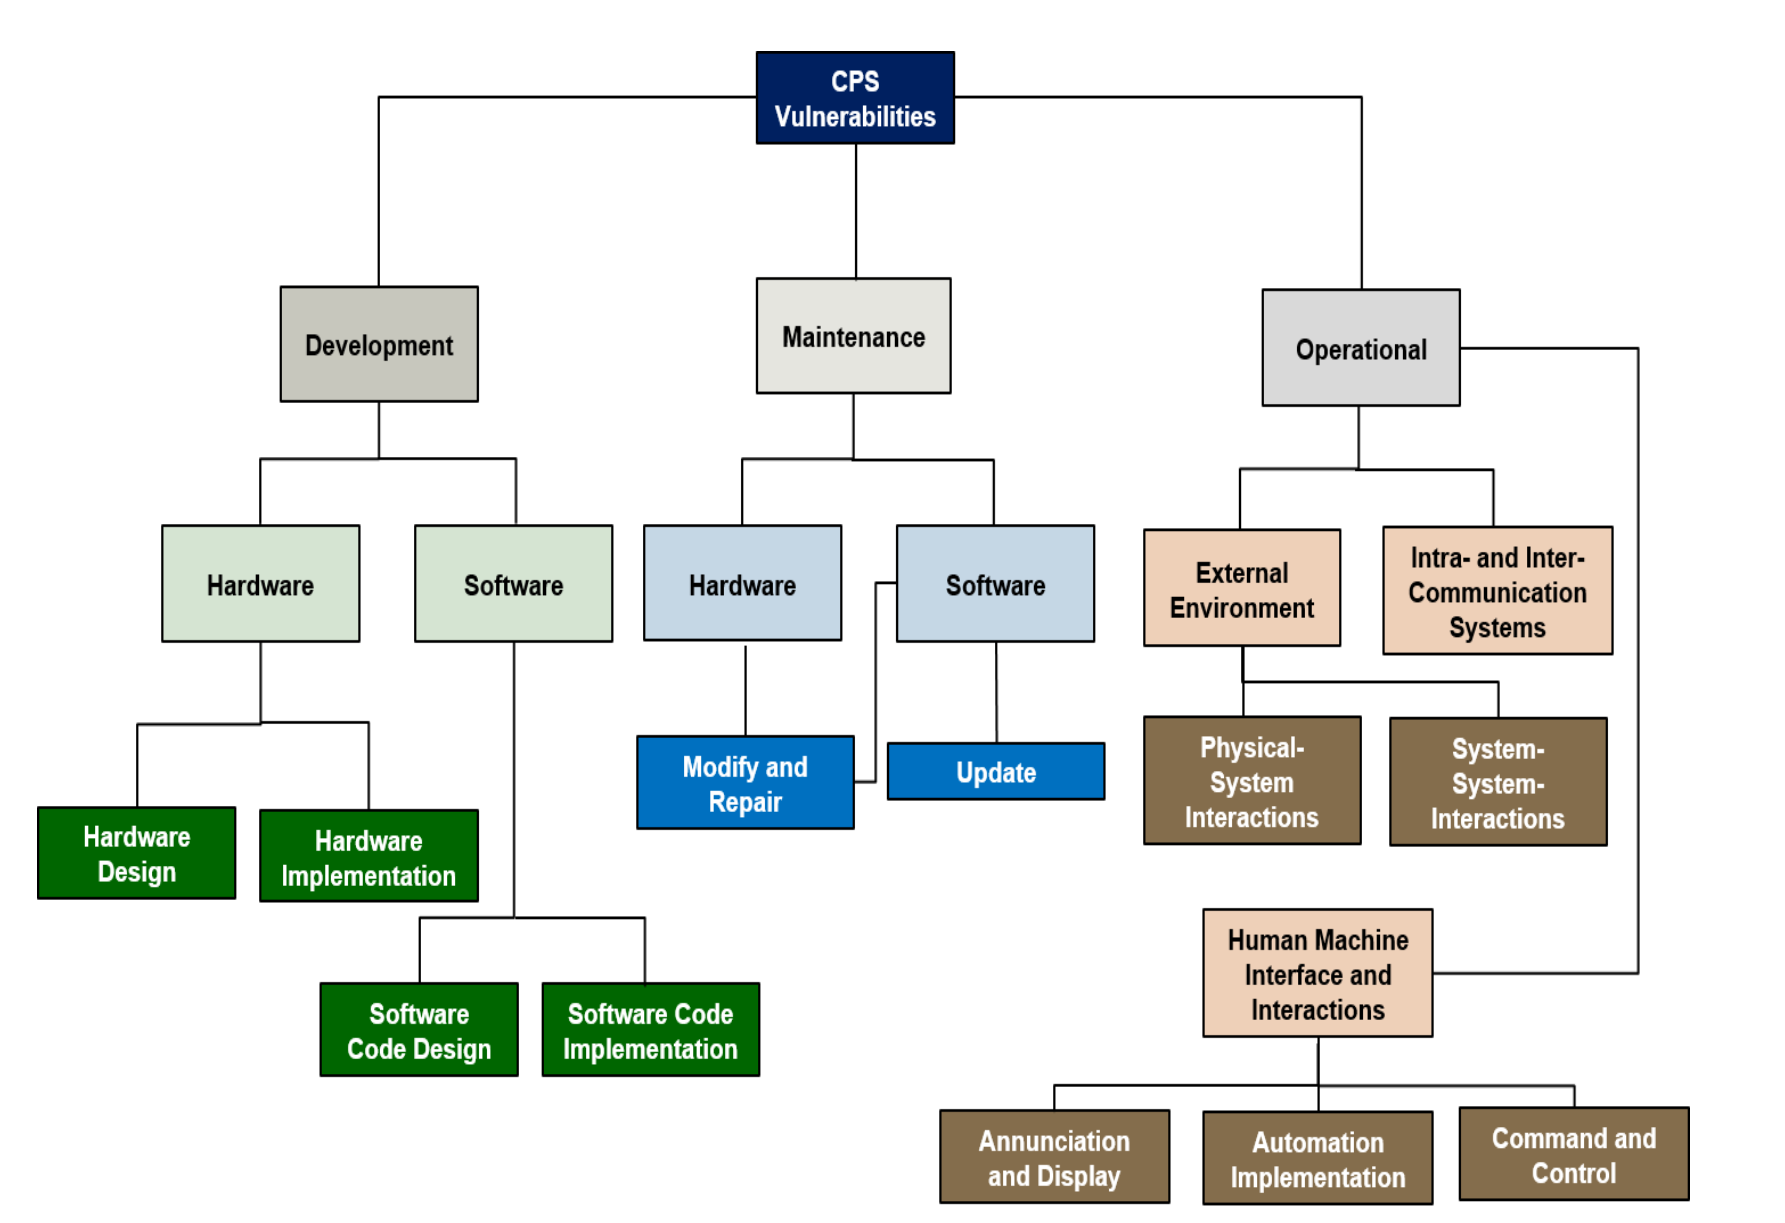
\includegraphics{images/07/cpsVulns.png}
	\caption{CPS Vulnerabilidades taxonomía}
	\label{fig:07/cpsVulns}
\end{figure}

A la izquierda de la figura \ref{fig:07/cpsVulns} hay una lista de vulnerabilidades son vulnerabilidades de plataforma, al centro hay vulnerabilidades de la gestión, y a la derecha vulnerabilidades operacionales.\\
Cómo hemos dicho antes, tipicamente es difícil actualizar el software para CPSs, esto es el motivo por el cual hay muchas vulnerabilidades relacionadas a la mantenimiento del software.

Las vulnerabilidades más comunes son:
\begin{itemize}
	\item Improper Input Validation / Validación incorrecta de las entradas
	\item Permissions, Privileges and Access Control / Permisos, privilegios y control de acceso
	\item Improper Authentication / Autenticación incorrecta
	\item Insufficient Verification of Data Authenticity / Verificación insuficiente de la autenticidad de los datos
	\item Poor Code Quality / Código de baja calidad
	\item Security Configuration and Maintenance / Configuración y mantenimiento de la seguridad
	\item Credentials Management / Gestión de credenciales
\end{itemize}

\subsection{Vulnerabilidades más comunes}
La más explotada vulnerabilidad en CPSs es \textbf{Buffer Overflow}, que es tipicamente permitida por la falta de validación de las entradas: los programadores suelen tener en cuenta lo que debería ocurrir y lo que podría ocurrir por error, pero no todas las posibilidades maliciosas.

Malas prácticas de código permiten a los atacantes suministrar datos inesperados y modificar así la ejecución del programa. Esta vulnerabilidad se llama \textbf{Lack of Bounds Checking}.


\textbf{Cross-Site scripting} vulnerabilidades pueden ser explotadas para muchos tipos de ataques, como el \textbf{Cross-Site Request Forgery} (CSRF), que permite a un atacante ejecutar comandos en el contexto de un usuario autenticado. En general, el Cross-Site Scripting permite \textbf{Code Injection}. 

\section{Vulnerabilities Assessment}
Para los CPS, los objetivos de seguridad están en orden inverso de prioridad, siendo la disponibilidad considerada la más importante, en lugar de la confidencialidad. El personal de la industria a menudo usa el término "seguridad" para referirse a la disponibilidad y fiabilidad del sistema.

Nada debe hacerse en una red CPS activa que pueda interferir o interrumpir las operaciones críticas del sistema. En el entorno CPS, los objetivos de seguridad del mundo IT son reemplazados por la salud y seguridad humana, la disponibilidad del sistema, y la puntualidad e integridad de los datos. Esta es la principal diferencia entre las evaluaciones de seguridad de CPS y de IT.

Esta diferencia también se aplica a las estrategias de mitigación. Ninguna solución de ciberseguridad puede implementarse en la red CPS si interfiere con la respuesta del sistema. El equipo de evaluación cibernética debe trabajar con el personal de la industria y los proveedores para realizar una evaluación efectiva sin comprometer la seguridad, disponibilidad o integridad del CPS.

CPS Vulnerabilities Assessment Execution Phases:
\begin{enumerate}
	\item \textbf{Reconnaissance} -
	The first part of a cyber security assessment is to identify a
target to attack.
	\item \textbf{Exploration} -
	Once a target has been identified, the assessment team attacks
the system
	\item \textbf{Exploit development} -
	Once a problem has been identified, the assessment team may
optionally develop an exploit for the vulnerability.
\item[] All these phases have specific aspects in CPS vulnerabilities assessment
\end{enumerate}

\subsection{Intrusion detection}

HIDS no se utilizan mucho en ICSs, porque ---tipicamente--- no se puede instalar software sobre CPS components.
Entonces, se utilizan \textbf{Network IDS} basados sobre \textbf{anomalias}.
La detección por firmas (signature-based) tiene buena precisión para IT sistemas, pero no lo es para ICSs, porque \dots // TODO

La detección por firmas (signature-based) tiene buena precisión para IT sistemas, pero no lo es para ICSs, porque tiene que depender de firmas conocidas y actualizadas, mientras que los protocolos y comportamientos en entornos ICS son muy específicos y a menudo propietarios.

% \subsection{Lateral Movements}

\textbf{Lateral Movements} son muy comunes en ICSs, porque los atacantes pueden moverse lateralmente a través de la red para obtener acceso a otros sistemas, y entonces, \textbf{honeypots} son una defensa muy eficaz para detectar y monitorear estos movimientos. Los honeypots simulan componentes legítimos del sistema, atrayendo a los atacantes y permitiendo analizar sus técnicas sin comprometer los sistemas reales.

La segmentación de la red, junto con controles de acceso estrictos entre zonas, también es fundamental para limitar la capacidad de los atacantes de moverse lateralmente una vez que han comprometido un punto de entrada inicial en la red ICS.

\subsection{Exploits mitigación}

En general es muy difícil mitigar los exploits en CPSs, porque no se pueden aplicar parches a los sistemas.

% // TODO



